\documentclass{beamer}
\usepackage[utf8]{inputenc}
\usepackage[spanish]{babel}
\usepackage{amsmath}
\usepackage{graphicx}

\title{Medición de Distancias con la Ley del Inverso Cuadrado}
\author{Manuel A. García \\ \texttt{mangarciama@unal.edu.co}}
\date{}

\begin{document}

\frame{\titlepage}

\begin{frame}{Introducción}
\begin{itemize}
    \item La ley del inverso cuadrado relaciona flujo (\(F\)) y distancia (\(d\)):
    \[
    F = \frac{L}{4\pi d^2}
    \]
\end{itemize}
\end{frame}

\begin{frame}{Montaje Experimental}
\begin{itemize}
    \item Cámara Nikon D5600 a 23.6 m de la primera lámpara.
    \item Imágenes tomadas en formato RAW y procesadas en FITS.
    \item Análisis fotométrico con \texttt{SAOImageDS9}.
\end{itemize}
\begin{figure}[H]
    \centering
    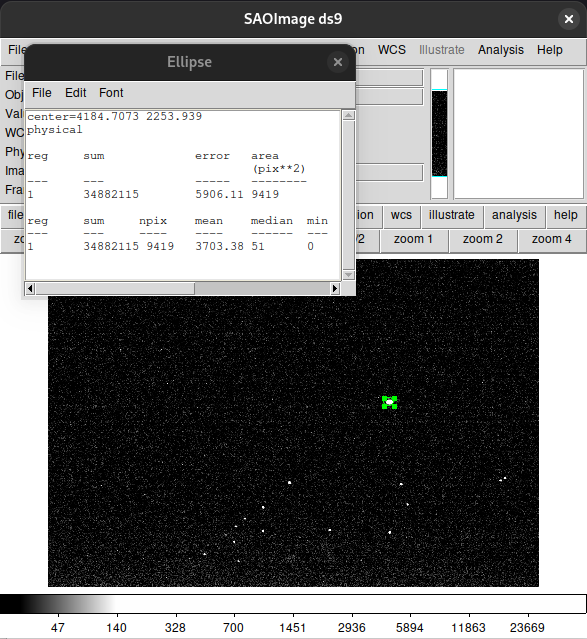
\includegraphics[width=0.45\textwidth]{ds9.png}
    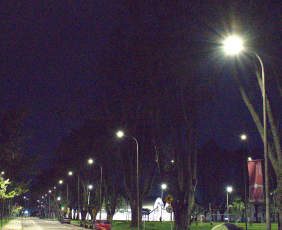
\includegraphics[width=0.5\textwidth]{lamp_reference.png}
    \caption{Análisis de brillo en \texttt{SAOImageDS9}.}
\end{figure}
\end{frame}

\begin{frame}{Ecuaciones Relevantes}
\begin{itemize}
    \item Flujo corregido:
    \[
    F_{\text{obj}} = F_0 - p_{\text{bg}} \cdot A
    \]
    \item Distancia preliminar:
    \[
    d(i) = d(1) \cdot \sqrt{\frac{F(1)}{F(i)}}
    \]
    \item Distancia corregida:
    \[
    d(i) = d_{\text{ref}} \cdot \sqrt{\frac{r(i) \cdot F(1)}{F(i)}}, \quad r(i) = \frac{L(i)}{L(1)} = \frac{d(i)^2 F(i)}{d(1)^2 F(1)}
    \]
\end{itemize}
\end{frame}

\begin{frame}{Resultados: Farolas}
  \begin{table}[H]
  \centering
  \begin{tabular}{|c|c|c|c|c|}
  \hline
  \textbf{\# Lampara} & \textbf{F\_mean} & \textbf{F\_bg\_mean} & \textbf{Area} $[px^2]$ & \textbf{d\_real} $[m]$ \\ \hline
  1 & 6474.11 & 11.24 & 5378 & 23.6 \\ \hline
  2 & 432.81  & 9.22  & 1618 & 47.6 \\ \hline
  3 & 192.97  & 10.30 & 1235 & NaN  \\ \hline
  4 & 136.15  & 11.13 & 756  & NaN  \\ \hline
  5 & 108.89  & 10.81 & 832  & NaN  \\ \hline
  6 & 44.75   & 11.26 & 538  & NaN  \\ \hline
  7 & 21.87   & 11.15 & 541  & NaN  \\ \hline
  8 & 22.10   & 10.14 & 486  & NaN  \\ \hline
  \end{tabular}
  \caption{Tabla de datos las mediciones.}
  \label{tab:lamps}
  \end{table}
\end{frame}


\begin{frame}{Resultados: Farolas}
\begin{table}[H]
\centering
\begin{tabular}{|c|c|c|c|c|c|c|}
\hline
\textbf{d\_real} & \textbf{F\_obj} & \textbf{d\_prelim} & \textbf{error\%} & \textbf{r} & \textbf{d\_adjusted} & \textbf{error\%} \\ \hline
23.60 & 6462.87 & 23.06 & 2  & 1.00 & 23.06 & 2  \\ \hline
44.10 & 423.59  & 90.07 & 104 & 0.21 & 41.24 & 6  \\ \hline
64.60 & 182.67  & 137.16 & 112 & 0.19 & 60.18 & 6  \\ \hline
85.10 & 125.02  & 165.80 & 94  & 0.23 & 79.63 & 6  \\ \hline
105.60 & 98.09  & 187.18 & 77  & 0.28 & 99.11 & 6  \\ \hline
126.10 & 33.49  & 320.33 & 154 & 0.16 & 129.25 & 2  \\ \hline
146.60 & 10.72  & 566.22 & 286 & 0.11 & 185.07 & 26 \\ \hline
167.10 & 11.96  & 535.98 & 220 & 0.14 & 200.27 & 19 \\ \hline
\end{tabular}
\caption{Datos de las lámparas con distancias reales, preliminares y ajustadas.}
\label{tab:analisis}
\end{table}
\end{frame}



\begin{frame}{Resultados: Farolas}
\begin{figure}[H]
    \centering
    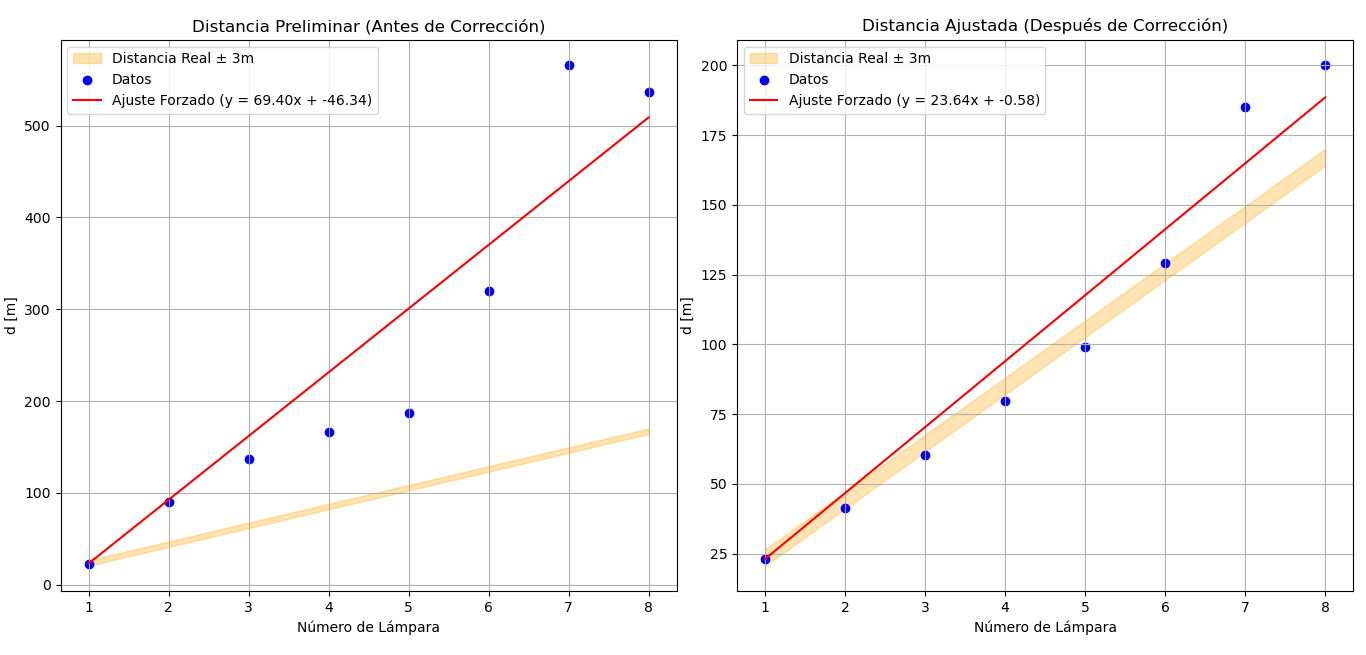
\includegraphics[width=0.95\textwidth]{grafica_analisis.png}
\end{figure}
\end{frame}



\begin{frame}{Resultados: Verificación Ley del Inverso Cuadrado (LED)}
\begin{table}[H]
\centering
\begin{tabular}{|c|c|c|c|c|c|}
\hline
F\_mean & F\_bg & Area $[px]$ & d\_real $ [cm] $ & d\_prelim $ [cm] $ & error\% \\ \hline
14171.60 & 49.42   & 29433 & 20.00  & 20.00 & 0.00  \\ \hline
18692.70 & 84.19   & 13258 & 30.00  & 25.96 & 13.47 \\ \hline
11127.90 & 44.03   & 12922 & 40.00  & 34.07 & 14.82 \\ \hline
6716.28  & 42.48   & 12816 & 50.00  & 44.09 & 11.82 \\ \hline
6404.19  & 40.53   & 9265  & 60.00  & 53.10 & 11.49 \\ \hline
5130.12  & 36.68   & 8446  & 70.00  & 62.17 & 11.19 \\ \hline
4493.05  & 37.63   & 7494  & 80.00  & 70.57 & 11.79 \\ \hline
3143.30  & 39.34   & 8419  & 90.00  & 79.76 & 11.37 \\ \hline
\end{tabular}
\caption{Datos de las lámparas con distancias reales y las calculadas por la ley del inverso cuadrado.}
\label{tab:analisis2}
\end{table}
\end{frame}




\begin{frame}{Resultados: Verificación Ley del Inverso Cuadrado (LED)}
\begin{figure}[H]
    \centering
    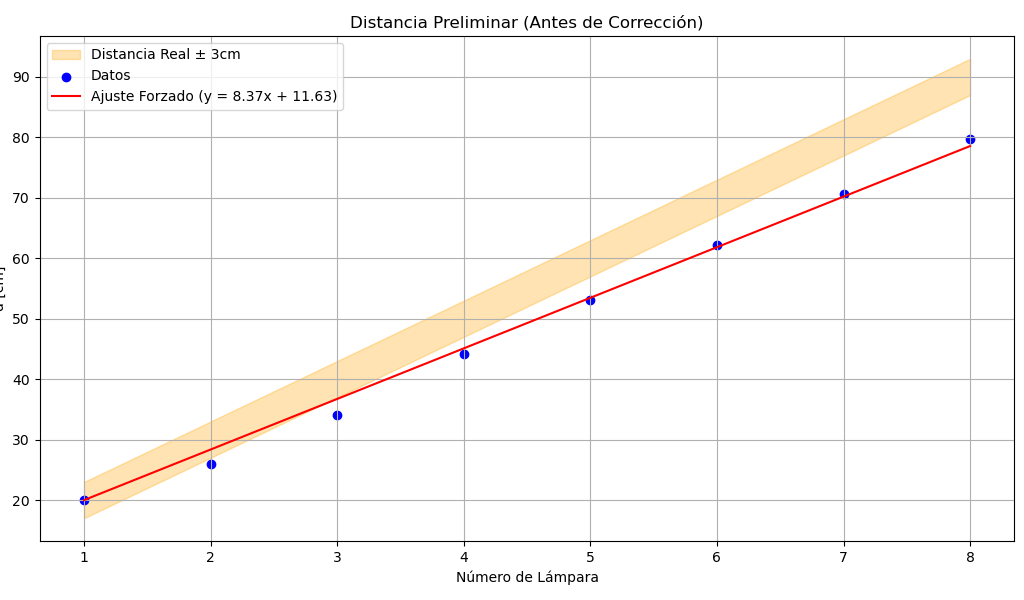
\includegraphics[width=0.8\textwidth]{grafica_analisis2.png}
    \caption{Errores en la medición de distancias con un LED.}
\end{figure}
\end{frame}

\begin{frame}{Conclusiones}
\begin{itemize}
    \item La ley del inverso cuadrado es válida, pero requiere correcciones en entornos reales.
    \item Las correcciones reducen errores significativos:
    \begin{itemize}
        \item Farolas: de \(286\%\) a \(26\%\).
        \item LED: errores promedio de \(11.7\%\).
    \end{itemize}
\end{itemize}
\end{frame}

\begin{frame}{Referencias}
  \nocite{*}
  \bibliographystyle{plain}
  \bibliography{references}
\end{frame}

\end{document}
